\section{Reconstruction for VLA Observations}

Compressed Sensing Reconstruction used on two different tasks:
\begin{itemize}
	\item Center detection on sunburst data
	\item Reconstruction from incomplete measurements of Supernova Remnant G55
\end{itemize}

Two different problems. One is the 

Structure potentially smaller than the primary beam.



\subsection{Sunburst Center Detection}

Sub- Primary Beam.
CS Objective Function

Figure: Dirty Map Peak, CLEAN, Single Peak Clean, Single Peak CS Reconstruction

\begin{figure}
	
\end{figure}

Wider Variance


\subsection{Reconstruction of Supernova Remnant G55}
\begin{figure}[h]
	\centering
	\begin{subfigure}[b]{0.45\linewidth}
		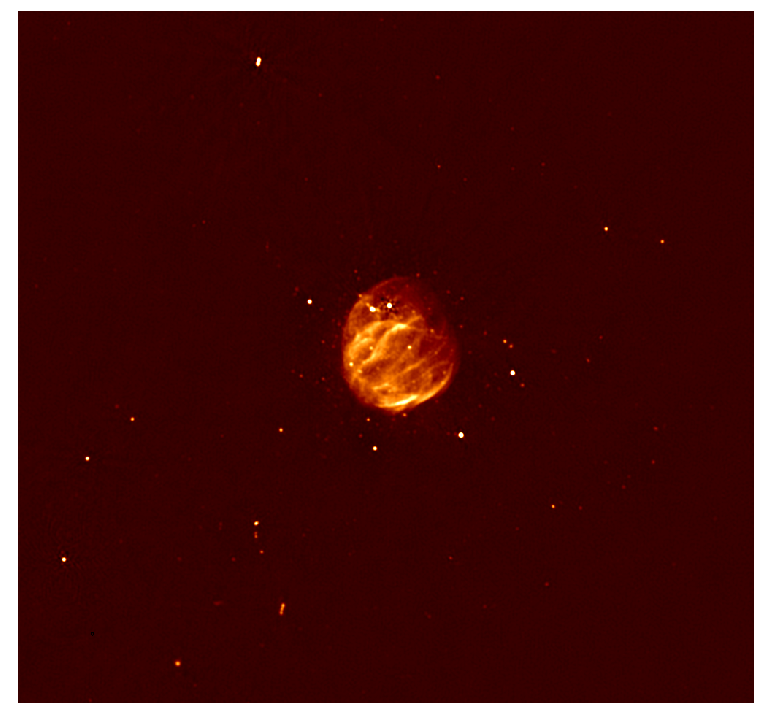
\includegraphics[width=\linewidth, trim={230px 210px 225px 200px}, clip]{./chapters/05.results/pic_G55_7.png}
		\caption{Reconstruction by NRAO.  Source:\cite{nraoG55}}
		\label{results:g55:nrao:rec}
	\end{subfigure}
	\begin{subfigure}[b]{0.45\linewidth}
		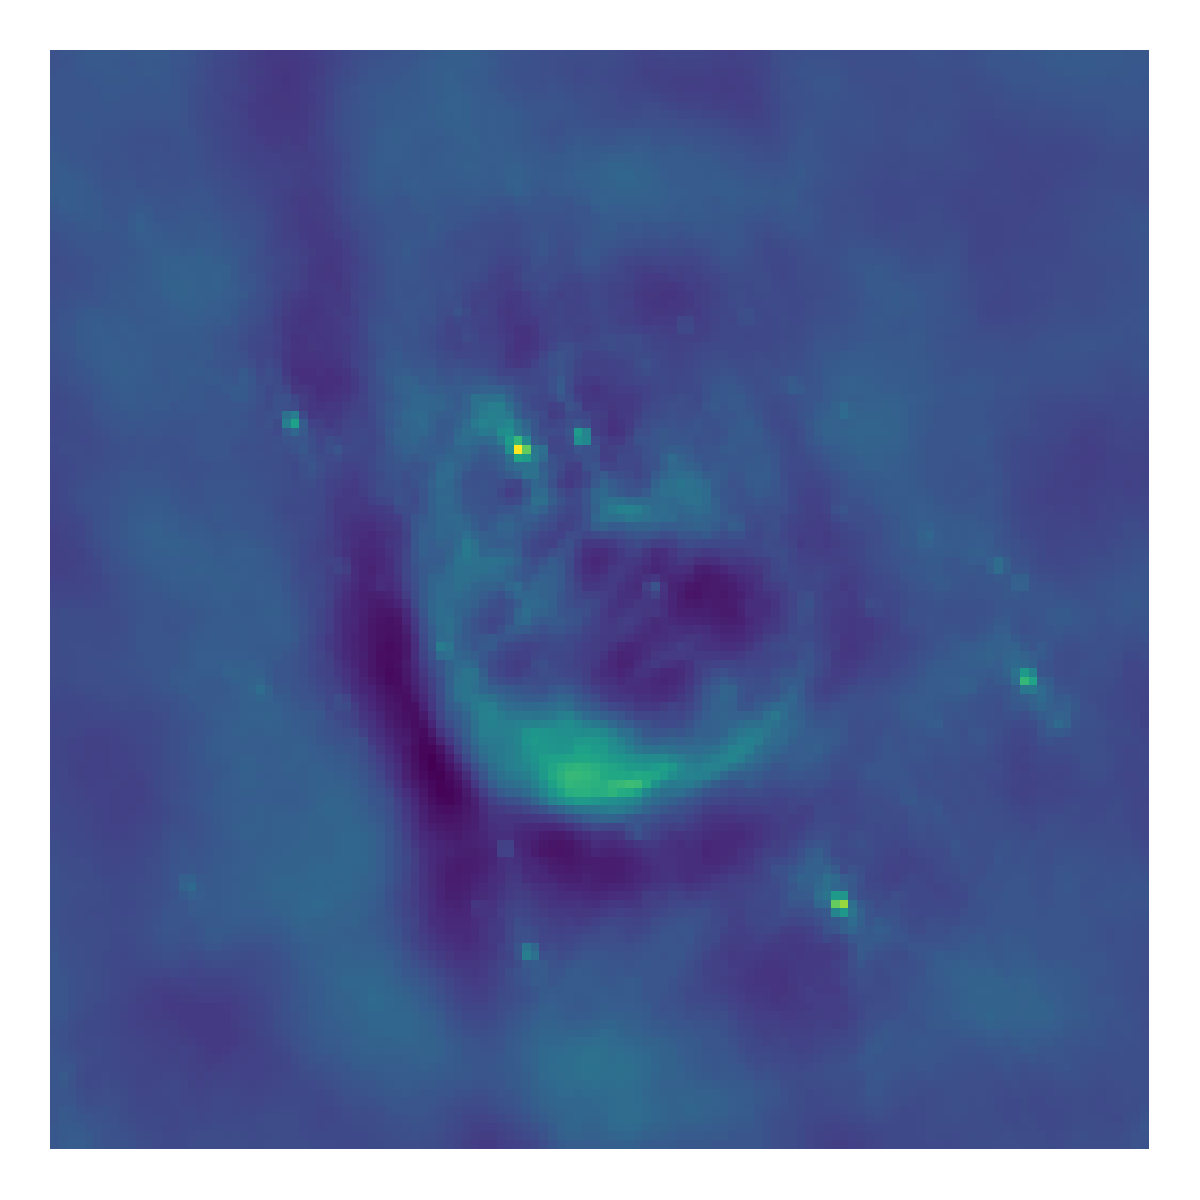
\includegraphics[width=\linewidth, trim={18px 19px 18px 18px}, clip]{./chapters/05.results/g55/raw_image.png}
		\caption{Dirty Image}
		\label{results:g55:nrao:dirty}
	\end{subfigure}
	\caption{SNR G55 source observed by VLA.}
	\label{results:g55:nrao}
\end{figure}

The supernova remnant (SNR) G55 was observed by VLA. 10 seconds of the 8 hour observation is publicly available through the CASA imaging tutorial\cite{casaImagingGuide}. \ref{results:g55:nrao:dirty} is the dirty image calculated from the 10 second observation. The full 8 hours are not readily available. The image \ref{results:g55:nrao:rec} is a reconstruction from an unknown VLA observation. The deconvolution algorithm is also unknown. For this project, the reconstructed image is assumed to show the true image of the sky.

\ref{results:g55:nrao} shows G55 to be a slightly "egg shaped" extended emission with six strong point sources. Several fainter point sources are inside and around the egg shaped extended emission. The dirty image \ref{results:g55:nrao:dirty} shows a corrupted version of G55. The six strong point sources are clearly visible as are the brighter parts of the extended emission. The dirty image also shows a negative "trench" striking through the image as well as brighter regions around the remnant. 

The size of the images \ref{results:g55:nrao} is about twice the size of the primary beam (the primary beam is approximately the size of the extended emission). In the real world, wide field imaging would be used. In this project, small field of view imaging was used because it is quicker to compute. 
It limits the dynamic range of the dirty image, the whole task gets harder. 

The CLEAN algorithm gets compared to Compressed Sensing Reconstructions. The parameters of CLEAN were taken from the CASA imaging tutorial\cite{casaImagingGuide}. The reconstructed images of Compressed Sensing are constrained to have no negative pixels. Negative pixels are not physically plausible and was shown to improve Compressed Sensing reconstructions for synthetic data\cite{mcewen2011compressed}. In total six different priors were tested with the analysis objective:
\begin{enumerate}
	\item No Regularization
	\item L1
	\item L2
	\item L1+L2
	\item Total Variation
	\item Starlet Transform
\end{enumerate}

The regularization parameter $\lambda$ needs to be estimated for each prior. The Miller\cite{miller1970least} $\lambda$ estimation was used and is shown in equation \eqref{results:eq:miller}. [Estimation of the noise level $e$, divided and $E$]. An approximate solution is needed to define the noise level and the amount of regularization. In this project, the result with no regularization was used for the $\lambda$ estimation.

This is not an ideal estimation, the image effectively gets reconstructed twice. Other Compressed Sensing Reconstructions approximate $x$ of equation \eqref{results:eq:miller} by running their optimizer a couple of iterations without regularization, which reduces the computational costs. 

\begin{equation}\label{results:eq:miller}
	\lambda \approx e / E \qquad  \left \| I_{dirty} - x \star PSF \right \|_2^2 \le e \qquad p(x) \le E
\end{equation}

Two figures compare the Dirty Image, CLEAN and the Compressed Sensing Reconstrutions. Figure \ref{res:g55:img} shows the reconstructed images on the same intensity scale. Figure \ref{res:g55:profile} shows the flux profile of a cut through the reconstructed images. The Cut through the remnant is located in the center of the profile image.

\begin{figure}[h]
	\centering
	\begin{subfigure}[b]{0.24\linewidth}
		\centering{Dirty Image}
		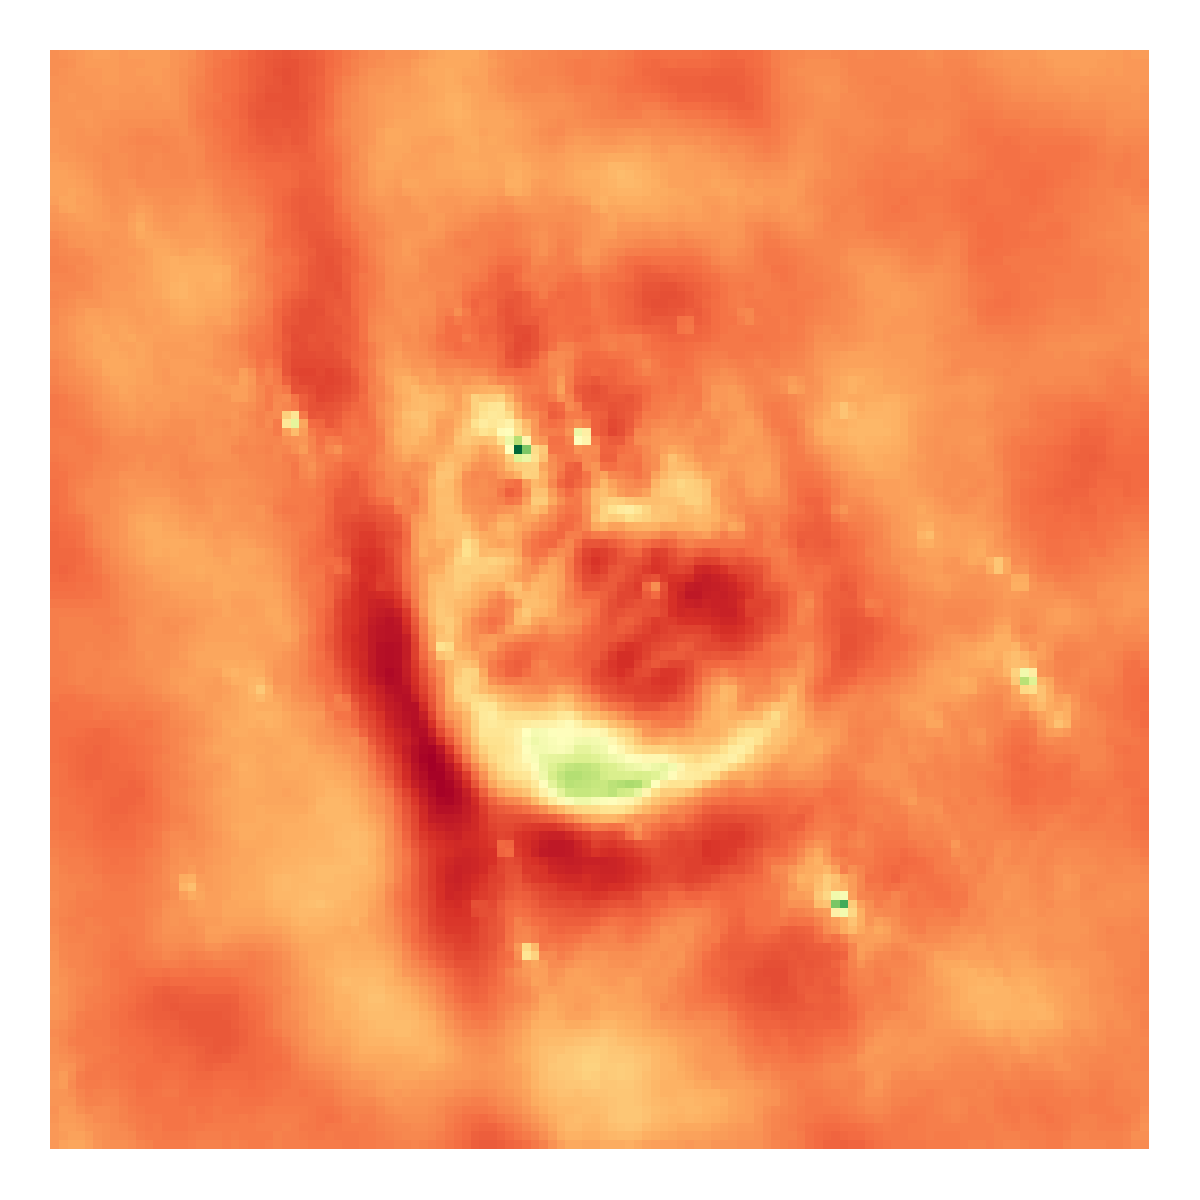
\includegraphics[width=\linewidth, trim={18px 19px 18px 18px}, clip]{./chapters/05.results/g55/raw_model.png}
	\end{subfigure}
	\begin{subfigure}[b]{0.24\linewidth}
		\centering{CLEAN}
		
\includegraphics[width=\linewidth, trim={18px 19px 18px 18px}, clip]{./chapters/05.results/g55/clean_model.png}
	\end{subfigure}
	\begin{subfigure}[b]{0.24\linewidth}
		\centering{No Regularization}
		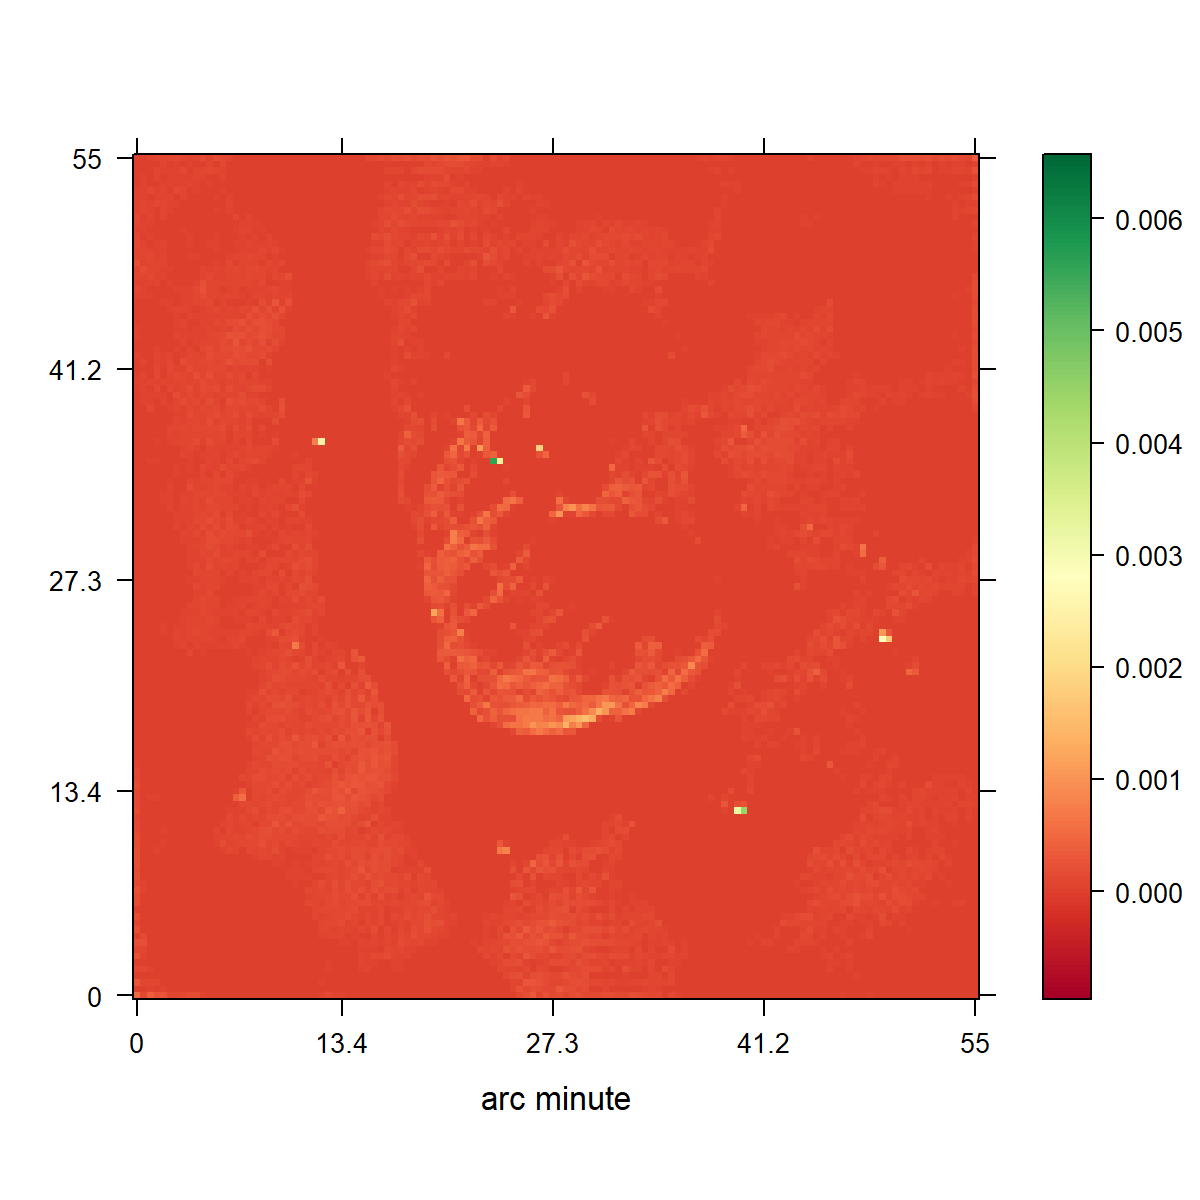
\includegraphics[width=\linewidth, trim={18px 19px 18px 18px}, clip]{./chapters/05.results/g55/positive_deconv_model.png}
	\end{subfigure}
	\begin{subfigure}[b]{0.24\linewidth}
		\centering{L1}
		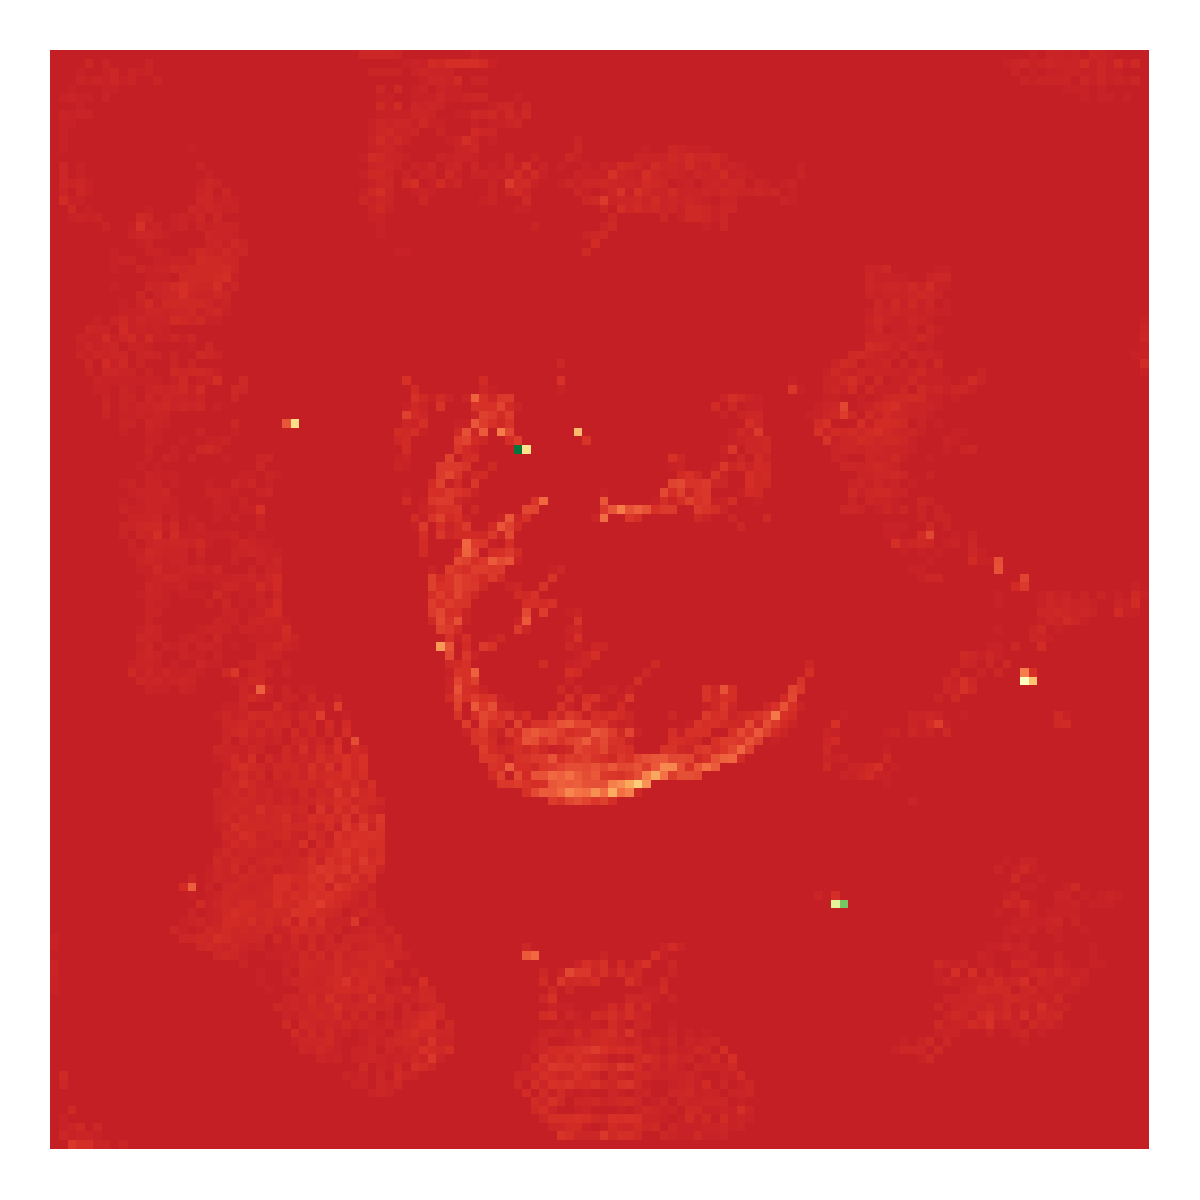
\includegraphics[width=\linewidth, trim={18px 19px 18px 18px}, clip]{./chapters/05.results/g55/L1_model.png}
	\end{subfigure}
	
	\begin{subfigure}[b]{0.24\linewidth}
		\vspace{10pt}
		\centering{L2}
		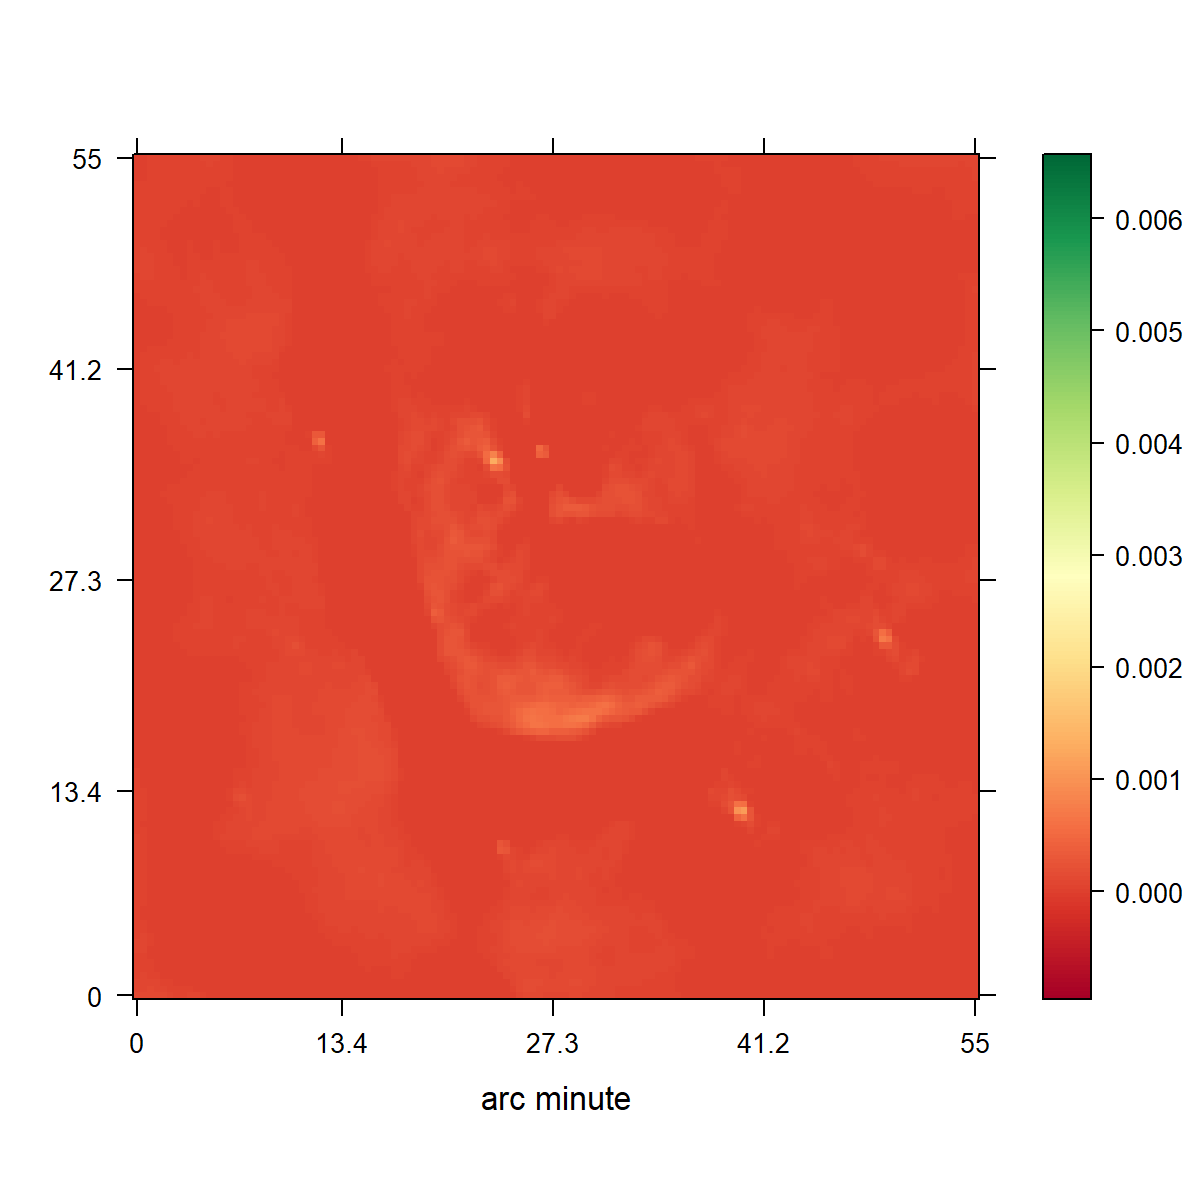
\includegraphics[width=\linewidth, trim={18px 19px 18px 18px}, clip]{./chapters/05.results/g55/L2_model.png}
	\end{subfigure}
	\begin{subfigure}[b]{0.24\linewidth}
		\centering{L1+L2}
		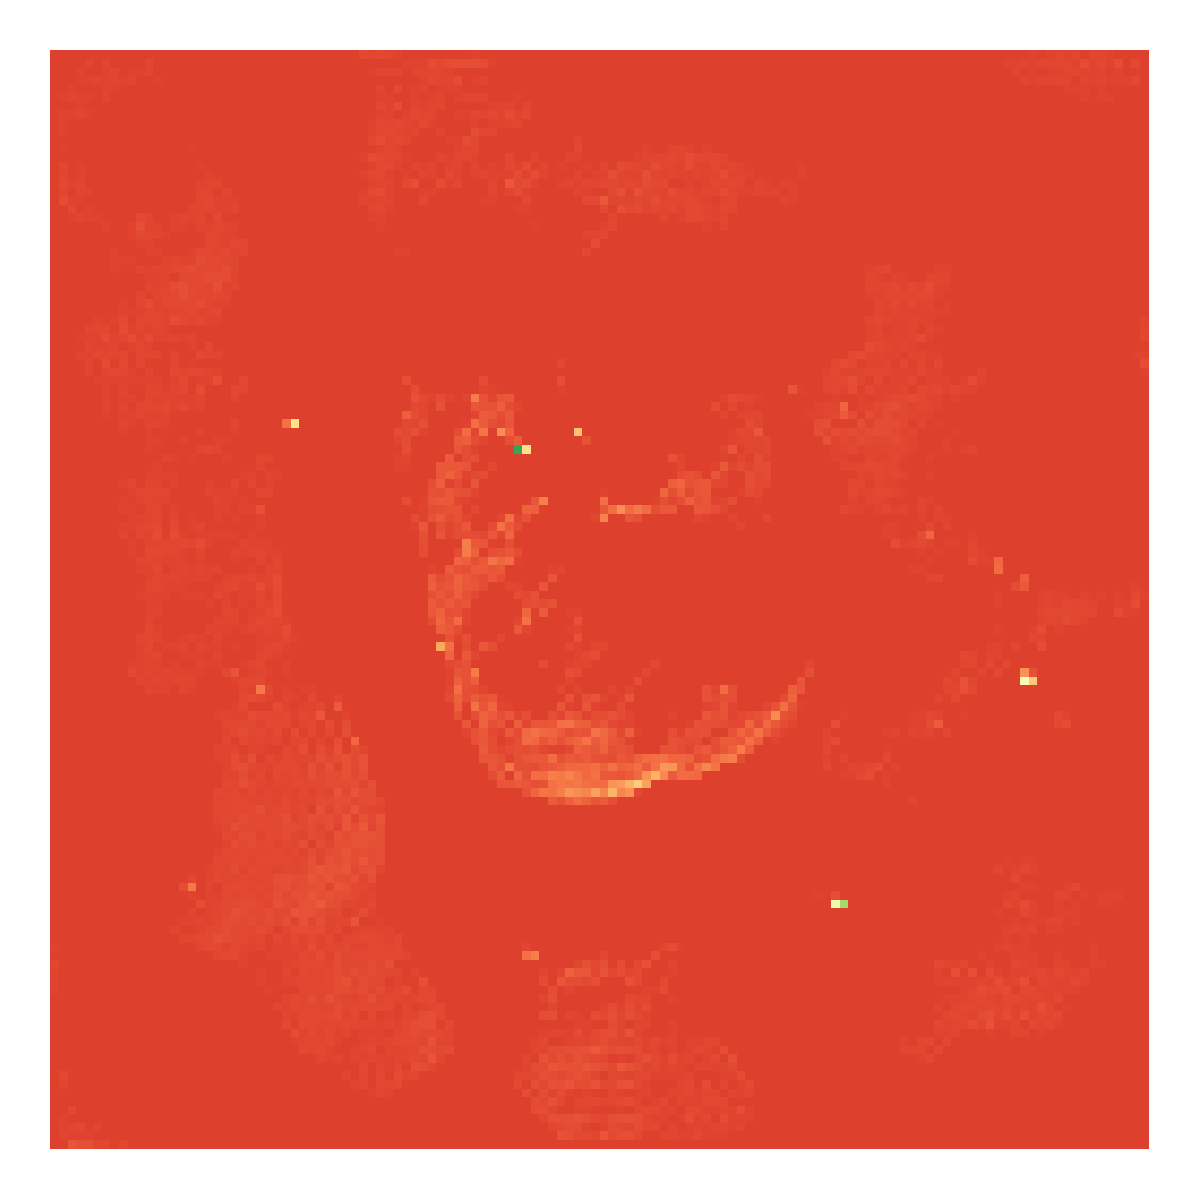
\includegraphics[width=\linewidth, trim={18px 19px 18px 18px}, clip]{./chapters/05.results/g55/L1+L2_model.png}
	\end{subfigure}
	\begin{subfigure}[b]{0.24\linewidth}
		\centering{Total Variation}
		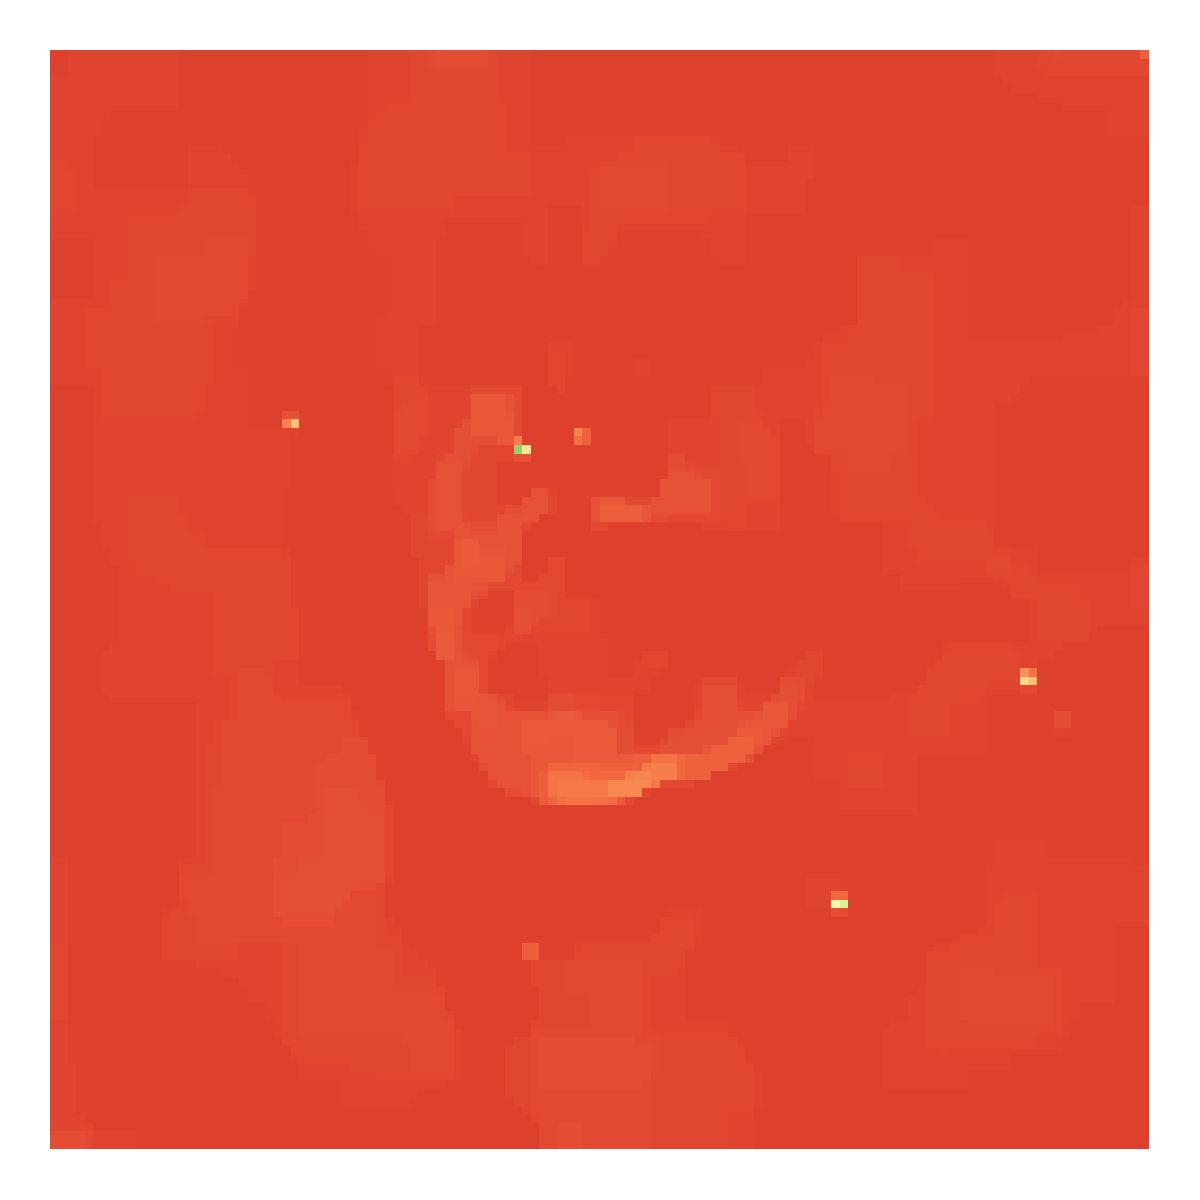
\includegraphics[width=\linewidth, trim={18px 19px 18px 18px}, clip]{./chapters/05.results/g55/TV_model.png}
	\end{subfigure}
	\begin{subfigure}[b]{0.24\linewidth}
		\centering{Starlets}
		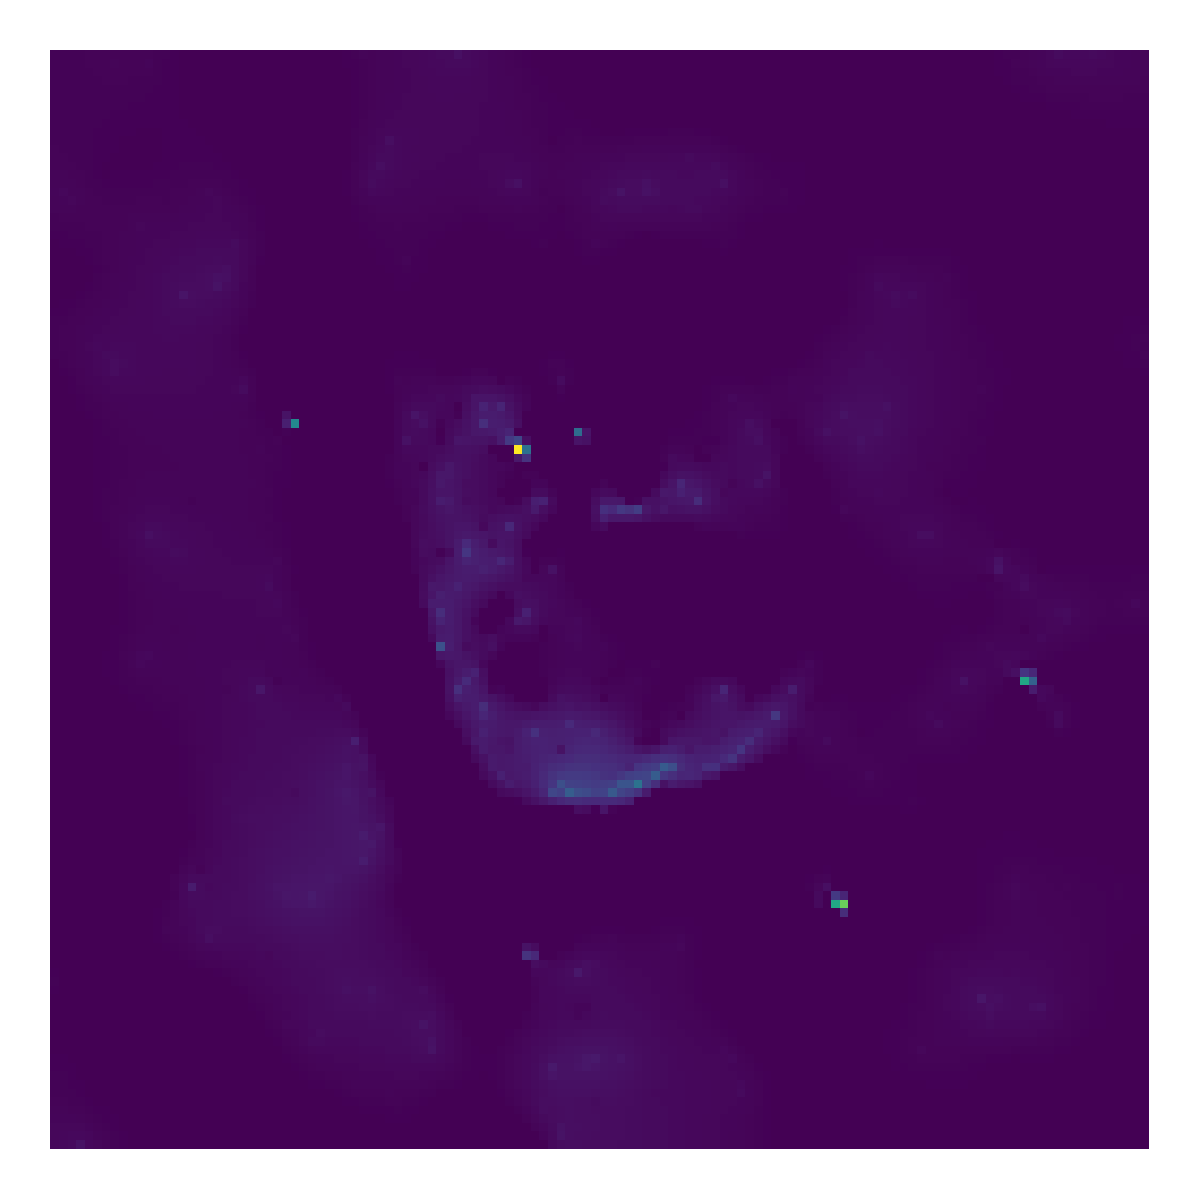
\includegraphics[width=\linewidth, trim={18px 19px 18px 18px}, clip]{./chapters/05.results/g55/starlets3_model.png}
	\end{subfigure}
	\caption{Reconstructed images of CLEAN and the different Compressed Sensing priors.} 
	\label{res:g55:img}
\end{figure}

\begin{figure}
	\centering
	\begin{subfigure}[b]{0.3\linewidth}
		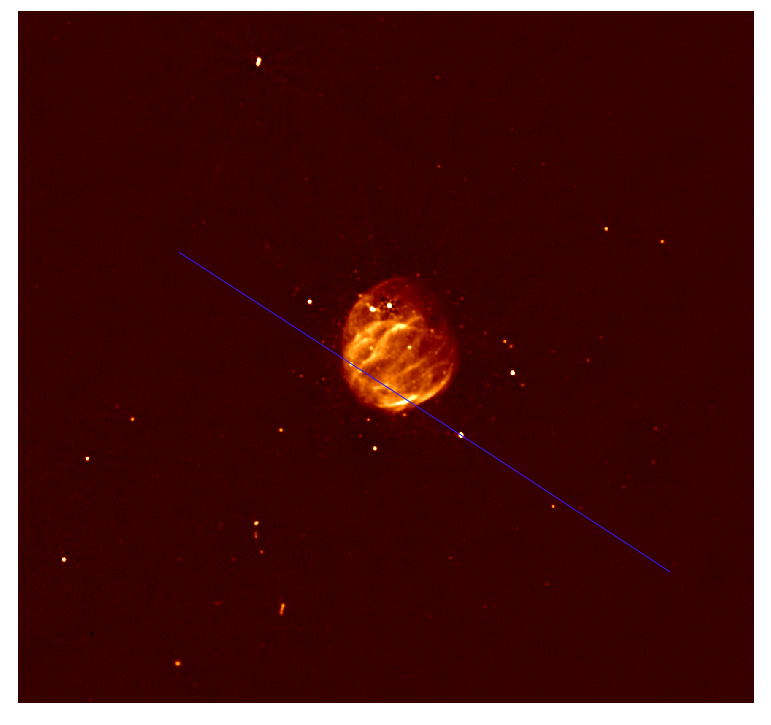
\includegraphics[width=\linewidth, trim={180px 170px 160px 136px}, clip]{./chapters/05.results/pic_G55_7_lined.png}
	\end{subfigure}
	\begin{subfigure}[b]{0.3\linewidth}
		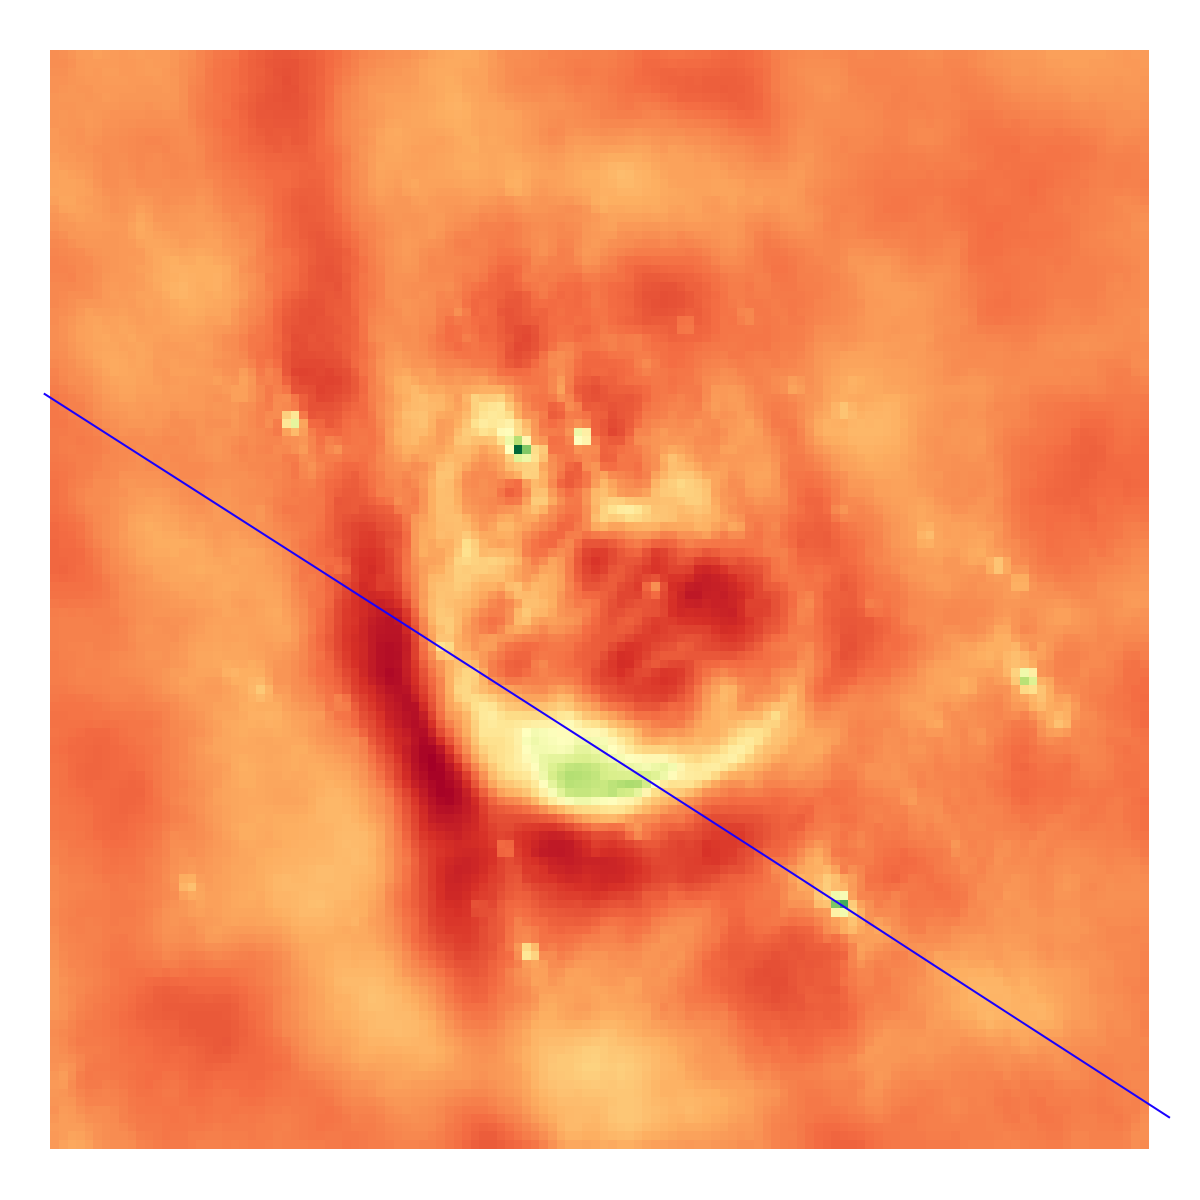
\includegraphics[width=\linewidth, trim={18px 19px 18px 18px}, clip]{./chapters/05.results/raw_image_lined.png}
	\end{subfigure}
	\caption{profile cut}
\end{figure}

\begin{figure}
	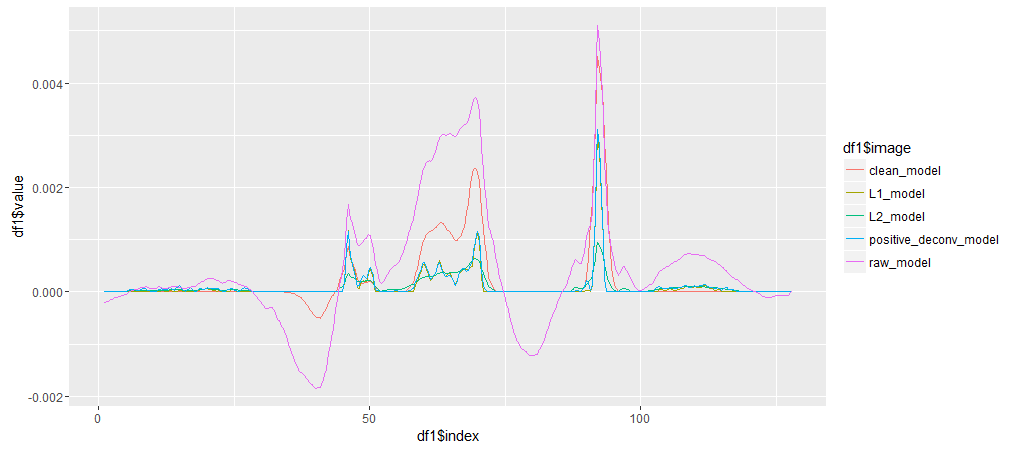
\includegraphics[width=\linewidth, clip]{./chapters/05.results/tmp0.png}
	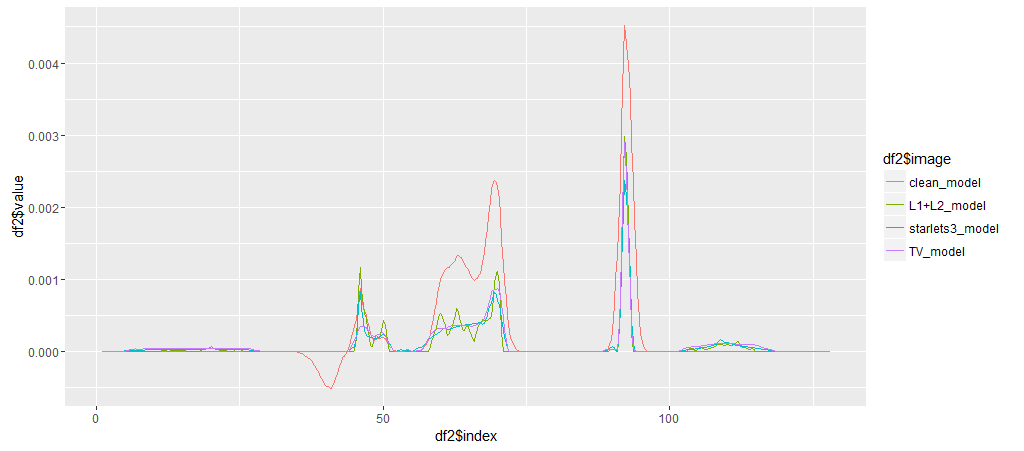
\includegraphics[width=\linewidth, clip]{./chapters/05.results/tmp1.png}
	\caption{Intensity profile of CLEAN and the different Compressed Sensing priors.}
	\label{res:g55:profile}
\end{figure}

\textbf{CLEAN:} CLEAN detects the brightest point sources, but finds only part of the extended emission. The top half of the "egg" emission is missing. The structures of the remnant are blurred compared to the Compressed Sensing reconstructions. With the parameters of the imaging tutorial, CLEAN models the trench as a region with negative emissions. This is not physically plausible, although the behaviour can be changed with additional parameters. The profile \ref{res:g55:profile} shows that CLEAN accurately reconstructs the flux of the large peaks, although the peaks are wider.

\textbf{No Regularization:} Detects the Egghead of the remnant and the non-negativity constraint keeps it from modelling the negative trench. It detects the smaller emissions around the remnant, but also detects "fake" extended emissions. The profile \ref{res:g55:profile} shows that the dirty image has a rise in flux at the borders of the image, which is likely an artefact of the measurement, considering it does not exist in the NRAO reconstruction \ref{results:g55:nrao:rec}. However, the the two smaller peaks in the center also appear in \ref{results:g55:nrao:rec} as do the two smaller point sources at the edge of the remnant. The ideal regularization would remove the "fake" extended emission around the remnant while keeping the plausible structure in the center.

\textbf{L1:} There is almost no visible difference between no regularization and L1. This is possibly an interaction with the Miller $\lambda$ estimation, since the result of no regularization was used to estimate the $\lambda$ of L1. The L1 regularization removes part of the "fake" extended emission, particularly in the top region, but also a few structures in the center. The peaks in the profile \ref{res:g55:profile} of L1 and no regularization are narrower than CLEAN, although they do not reach the same peak flux. L1 is prone to produce unlikely extended emissions: The "fake" emissions have a saw profile. If the emissions were real, the L1 regularization would produce artefacts.

\textbf{L2:} Forces the extended emissions to be more plausible, although it considerably lowers the flux of bright point sources. The profile \ref{res:g55:profile} shows L2 forces the bright peak to widen and lower. The peak is almost as wide as the CLEAN reconstruction. In the remnant center, it smoothers the two fainter peaks.

\textbf{L1+L2}: Since L1 does a good job with point sources, but needs to be more continuous for extended emissions, why does one not combine both regularizations? The flexibility of Compressed Sensing Reconstructions allows for it. In reality, Tradeoff between point sources and extended. How to chose the tradeoff is not trivial, here it was assumed to be  equal. In this example, all pixels are very close to zero (Maximum: 0.0076 in Dirty Image), Miller lambda estimation is dominated by the L1 term while the L2 term gets neglected. The larger the values in the dirty image, the more L2 dominates over L1. Combination is not trivial.

\textbf{Total Variation:} Simple prior that was used in Image denoising. Reduces the gradient over the whole image. [It tries to have as few changes in the image as possible.] The reconstructed image shows both extended emissions and point sources. It has trouble with point sources inside extended emissions. In this case it cuts off the point source and the peak in image \ref{} is not here.

\textbf{Starlets:} A more sophisticated try at combining both. smallest starlet is larger than the antenna beam width.



[No free lunch theorem.] The regularization decides what is noise and what is true. Search for regularization that finds the true image in every observation. CS is flexible and allows for a combination of regularization.

starlets finds a lot of smaller point sources, but they do
Size of scaling function.

CLEAN has the best flux reconstruction for point sources the beam even for point sources. L1 and L2 tradeoff. Try at combining both extended emissions and point sources.

Problem with memory, $x \star PSF$ gets modeled as a vector matrix multiplication $Px$. The image $x$ and $PSF$ with dimensions of $128 * 128$, result in a matrix of size $128^2 * 128^2$. The memory requirement scales quadratic with the number of pixels. 


